% !TEX program = xelatex
\documentclass[UTF8,fontset=fandol,a4paper,11pt]{ctexart}
\usepackage[margin=21mm,top=23mm,bottom=22mm,headheight=16pt]{geometry}
\usepackage{amsmath,amssymb,mathtools,bm}
\usepackage{tikz}
\usetikzlibrary{arrows.meta,calc,angles,quotes,patterns}
\usepackage{xcolor,booktabs,array,longtable,enumitem,fancyhdr,needspace}
\usepackage[unicode,hidelinks]{hyperref}
\definecolor{ink}{HTML}{24343C}
\definecolor{accent}{HTML}{166A70}
\definecolor{muted}{HTML}{65747A}
\definecolor{rulegray}{HTML}{D4DDE0}
\definecolor{warm}{HTML}{966037}
\color{ink}
\setlength{\parindent}{2em}
\setlength{\parskip}{4pt}
\linespread{1.12}
\AtBeginDocument{\setlength{\abovedisplayskip}{6pt plus 2pt minus 1pt}
\setlength{\belowdisplayskip}{6pt plus 2pt minus 1pt}
\setlength{\abovedisplayshortskip}{0pt plus 1pt}
\setlength{\belowdisplayshortskip}{4pt plus 1pt}}
\setlist[enumerate]{label=(\arabic*),leftmargin=2.3em,itemsep=3pt,topsep=4pt}
\setlist[itemize]{leftmargin=2em,itemsep=2pt,topsep=4pt}
\allowdisplaybreaks[1]
\setlength{\emergencystretch}{2em}
\setcounter{secnumdepth}{0}
\providecommand{\tightlist}{\setlength{\itemsep}{0pt}\setlength{\parskip}{0pt}}
\ctexset{section={format=\Large\bfseries\color{accent},beforeskip=10pt,afterskip=9pt},
subsection={format=\normalsize\bfseries\color{accent},beforeskip=10pt,afterskip=4pt},
subsubsection={format=\normalsize\bfseries,beforeskip=8pt,afterskip=3pt}}
\pagestyle{fancy}
\fancyhf{}
\fancyhead[L]{\small\color{muted}物理学难题集萃}
% 页眉仅保留书名；版本名称只在封面显示。
\fancyfoot[L]{\small\color{muted}\chapterlabel}
\fancyfoot[R]{\small\thepage}
\renewcommand{\headrulewidth}{0.4pt}
\renewcommand{\footrulewidth}{0pt}
\newcommand{\dd}{\mathop{}\!\mathrm{d}}
\newcommand{\vect}[1]{\bm{#1}}
\newcommand{\tagline}[1]{\noindent{\small\color{muted}#1}\par}
\newcommand{\result}[1]{\begin{equation*}\boxed{#1}\end{equation*}}
\newcommand{\figcaption}[1]{\par\vspace{2pt}{\small\color{muted}#1}\par}
\newcommand{\teach}[2]{\Needspace{4\baselineskip}\subsection*{讲解要点与追问}#1\par\smallskip\noindent\textbf{追问：}#2\par}
\newcommand{\workarea}{\par\vspace{7mm}\noindent{\small\color{muted}作答区}\par\vspace{4mm}
\noindent\textcolor{rulegray}{\rule{\linewidth}{0.3pt}}\par\vspace{16mm}
\noindent\textcolor{rulegray}{\rule{\linewidth}{0.3pt}}\par\vspace{16mm}
\noindent\textcolor{rulegray}{\rule{\linewidth}{0.3pt}}\par\vspace{16mm}
\noindent\textcolor{rulegray}{\rule{\linewidth}{0.3pt}}}
\tikzset{axis/.style={-{Stealth[length=2mm]},thin,color=muted},
motion/.style={-{Stealth[length=2.3mm]},thick,color=accent},
force/.style={-{Stealth[length=2.3mm]},thick,color=warm},
traj/.style={thick,color=accent},guide/.style={dashed,thin,color=muted},
object/.style={thick,color=ink},every node/.style={font=\small}}\widowpenalty=10000\clubpenalty=10000\displaywidowpenalty=10000\newcommand{\chapterlabel}{电磁学第二章\quad 磁场、磁介质}

\hypersetup{pdftitle={电磁学第二章 磁场、磁介质·学生版},pdfauthor={}}

\begin{document}

\pdfbookmark[0]{电磁学第二章 磁场、磁介质}{cover}

\thispagestyle{empty}\vspace*{22mm}
\noindent{\Huge\bfseries 物理学难题集萃}\par\vspace{10mm}
\noindent{\LARGE 电磁学第二章}\par\vspace{6mm}
\noindent{\LARGE 磁场、磁介质}\par\vspace{12mm}
\noindent{\Large\color{accent}学生版}\par\vspace{9mm}
\noindent\textcolor{accent}{\rule{\linewidth}{1pt}}\par\vspace{9mm}
\noindent 第1--27题\par\vfill\clearpage
\pdfbookmark[1]{题目目录}{contents}\section*{题目目录}
\begin{longtable}{@{}r p{113mm} r@{}}\toprule 题号 & 题目 & 页码\\\midrule

\hyperref[q:1]{1} & \hyperref[q:1]{半球面经线电流的球心磁场} & \pageref{q:1} \\

\hyperref[q:2]{2} & \hyperref[q:2]{抛物线形电流在焦点的磁场} & \pageref{q:2} \\

\hyperref[q:3]{3} & \hyperref[q:3]{均匀带电球面旋转的轴内磁场} & \pageref{q:3} \\

\hyperref[q:4]{4} & \hyperref[q:4]{无限长螺旋导线的轴上磁场} & \pageref{q:4} \\

\hyperref[q:5]{5} & \hyperref[q:5]{互补圆柱导体空隙中的均匀磁场} & \pageref{q:5} \\

\hyperref[q:6]{6} & \hyperref[q:6]{有限厚电流层的磁场分布} & \pageref{q:6} \\

\hyperref[q:7]{7} & \hyperref[q:7]{载流圆柱内的电子收缩与净电荷} & \pageref{q:7} \\

\hyperref[q:8]{8} & \hyperref[q:8]{磁场中转杆与滑动带电环} & \pageref{q:8} \\

\hyperref[q:9]{9} & \hyperref[q:9]{地磁场中带电圆环的滑动与纯滚动} & \pageref{q:9} \\

\hyperref[q:10]{10} & \hyperref[q:10]{电子枪击靶的圆轨道与螺旋轨道} & \pageref{q:10} \\

\hyperref[q:11]{11} & \hyperref[q:11]{平移细管内出射粒子追碰目标} & \pageref{q:11} \\

\hyperref[q:12]{12} & \hyperref[q:12]{方波轴向磁场中的电子束聚焦} & \pageref{q:12} \\

\hyperref[q:13]{13} & \hyperref[q:13]{同轴磁控管的临界磁场} & \pageref{q:13} \\

\hyperref[q:14]{14} & \hyperref[q:14]{点源到点像的磁场边界} & \pageref{q:14} \\

\hyperref[q:15]{15} & \hyperref[q:15]{电子束先会聚再扩束的四区磁场} & \pageref{q:15} \\

\hyperref[q:16]{16} & \hyperref[q:16]{环形磁场中的电子束聚焦与漂移} & \pageref{q:16} \\

\hyperref[q:17]{17} & \hyperref[q:17]{磁铁边缘场的单平面聚焦} & \pageref{q:17} \\

\hyperref[q:18]{18} & \hyperref[q:18]{电场漂移与磁场梯度漂移} & \pageref{q:18} \\

\hyperref[q:19]{19} & \hyperref[q:19]{重力与磁场中同高度的再相遇} & \pageref{q:19} \\

\hyperref[q:20]{20} & \hyperref[q:20]{载流双杆与弹簧的小振动} & \pageref{q:20} \\

\hyperref[q:21]{21} & \hyperref[q:21]{旋转带电圆环的附加张力} & \pageref{q:21} \\

\hyperref[q:22]{22} & \hyperref[q:22]{圆电流对共面长直导线的作用力} & \pageref{q:22} \\

\hyperref[q:23]{23} & \hyperref[q:23]{闭合稳恒电流回路间的作用与反作用} & \pageref{q:23} \\

\hyperref[q:24]{24} & \hyperref[q:24]{超导平板上方电流环的悬浮与振动} & \pageref{q:24} \\

\hyperref[q:25]{25} & \hyperref[q:25]{均匀磁化长棒侧面的场边界} & \pageref{q:25} \\

\hyperref[q:26]{26} & \hyperref[q:26]{均匀磁化球壳在球心的磁场} & \pageref{q:26} \\

\hyperref[q:27]{27} & \hyperref[q:27]{旋转径向极化圆柱的场能量} & \pageref{q:27} \\

\bottomrule\end{longtable}

\noindent 本章采用SI单位。$e>0$为电子电荷的绝对值，电子电荷为$-e$。图中$\odot$表示垂直纸面向外，$\otimes$表示垂直纸面向里；近似范围与其余符号在各题中说明。

\clearpage

\pdfbookmark[2]{第 1 题 半球面经线电流的球心磁场}{q1}

\section*{第 1 题\quad 半球面经线电流的球心磁场}\label{q:1}

半径为$R$的金属球面上，电流$2I$由南极流入、沿经线均匀分布后在北极流出，两端接沿极轴延伸的半无限长直导线。现沿过极轴的平面把球分成左右两半，移去右半球面；余下左半球面的电流分布保持不变，总电流为$I$。取极轴为$z$轴，左半球位于$y<0$，$x,y,z$构成右手坐标系。求球心$O$处的磁感应强度。

\begin{center}\begin{minipage}{.97\linewidth}\centering
\begin{tikzpicture}[x=1cm,y=1cm,font=\small]
\fill[accent!10] (0,-1.7) arc(-90:-270:1.7)--cycle;
\draw[object] (0,-1.7) arc(-90:-270:1.7);
\draw[guide] (0,-1.7)--(0,1.7);
\draw[axis] (0,0)--(2.7,0) node[right] {$y$};
\draw[axis] (0,0)--(0,2.85) node[above] {$z$};
\draw[motion] (0,-2.6)--(0,-1.75) node[midway,right] {$I$};
\draw[motion] (0,1.75)--(0,2.6) node[midway,right] {$I$};
\draw[motion] (-1.62,-.48) arc(-163:-197:1.7);
\node[left] at (-1.8,0) {$I:\ \mathrm S\to\mathrm N$};
\fill (0,0) circle(1.5pt) node[below right] {$O$};
\draw[<->] (0,0)--(-1.2,1.2) node[midway,above] {$R$};
\node at (1.8,-1.05) {$\odot\ +x$};
\node at (-.6,-2.95) {$yz$截面，保留$y<0$半球};
\end{tikzpicture}
\figcaption{图电2.1　过极轴的截面；箭头表示南极到北极的经线电流。切面为$y=0$，极轴两端接线均在球外。}
\end{minipage}\end{center}


\workarea

\clearpage

\pdfbookmark[2]{第 2 题 抛物线形电流在焦点的磁场}{q2}

\section*{第 2 题\quad 抛物线形电流在焦点的磁场}\label{q:2}

一根无限长细导线弯成抛物线，焦点到顶点的距离为$a$，通有恒定电流$I$。取抛物线为$x^2=4ay$，焦点$P=(0,a)$，电流从左支流向顶点，再沿右支流出。求$P$处的磁感应强度。

\begin{center}\begin{minipage}{.98\linewidth}\centering
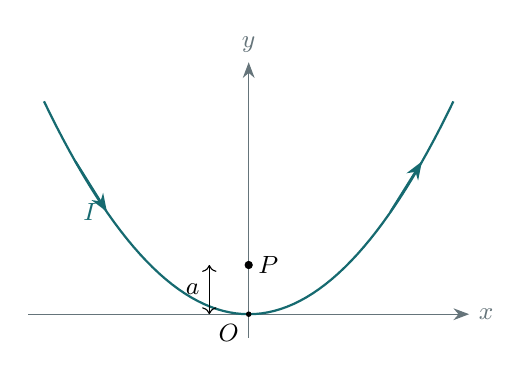
\begin{tikzpicture}[x=1cm,y=1cm]
\draw[axis] (-2.8,0)--(2.8,0) node[right] {$x$};\draw[axis] (0,-.3)--(0,3.2) node[above] {$y$};\draw[traj,domain=-2.6:2.6,samples=65] plot(\x,{.4*\x*\x});
\fill (0,0) circle(1pt) node[below left] {$O$};\fill (0,.625) circle(1.5pt) node[right] {$P$};\draw[<->] (-.5,0)--(-.5,.625) node[midway,left] {$a$};\draw[motion] (-2.2,1.94)--(-1.8,1.3) node[left] {$I$};\draw[motion] (1.8,1.3)--(2.2,1.94);
\end{tikzpicture}\figcaption{图电2.2　电流沿左支向下、右支向上。}\end{minipage}\end{center}

\workarea

\clearpage

\pdfbookmark[2]{第 3 题 均匀带电球面旋转的轴内磁场}{q3}

\section*{第 3 题\quad 均匀带电球面旋转的轴内磁场}\label{q:3}

半径$R$、面电荷密度$\sigma$的均匀带电球面，绕一条直径以角速度$\vect\omega=\omega\vect e_x$匀速旋转。证明：球内该直径上各点的磁感应强度相同，并求其值。

\begin{center}\begin{minipage}{.98\linewidth}\centering
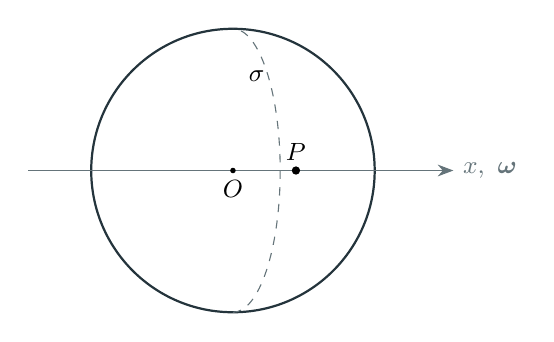
\begin{tikzpicture}[x=1cm,y=1cm]
\draw[object] (0,0) circle(1.8);\draw[axis] (-2.6,0)--(2.8,0) node[right] {$x,\ \vect\omega$};\draw[guide] (0,-1.8) arc(-90:90:.6 and 1.8);\fill (0,0) circle(1pt) node[below] {$O$};\node at (.3,1.2) {$\sigma$};\fill (.8,0) circle(1.5pt) node[above] {$P$};
\end{tikzpicture}\figcaption{图电2.3　旋转轴取水平x轴，P位于球内轴段。}\end{minipage}\end{center}

\workarea

\clearpage

\pdfbookmark[2]{第 4 题 无限长螺旋导线的轴上磁场}{q4}

\section*{第 4 题\quad 无限长螺旋导线的轴上磁场}\label{q:4}

真空中一根无限长细导线，沿半径$R$、螺距$H>0$的圆柱面绕成等距螺旋线，电流为$I$。圆柱轴为$y$轴。用参数$\phi$规定导线位置
\[
 \vect r(\phi)=(R\cos\phi,h\phi,R\sin\phi),\qquad h=H/(2\pi),
\]
电流沿$\phi$增大方向。求原点$O$处磁场的三个分量；说明轴上其他点的场怎样变化。

\begin{center}\begin{minipage}{.98\linewidth}\centering
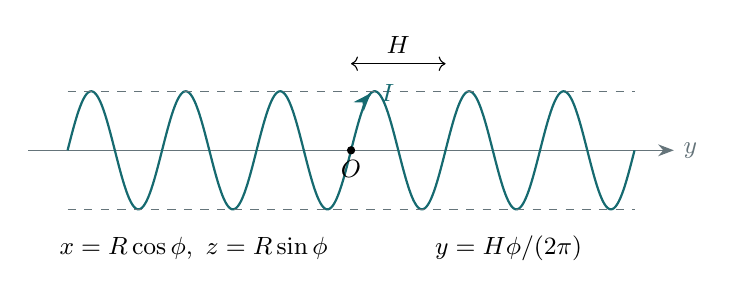
\begin{tikzpicture}[x=1cm,y=1cm]
\draw[axis] (-4.1,0)--(4.1,0) node[right] {$y$};\draw[traj,domain=-1080:1080,samples=360] plot({\x/300},{.75*sin(\x)});\draw[guide] (-3.6,.75)--(3.6,.75);\draw[guide] (-3.6,-.75)--(3.6,-.75);\draw[<->] (0,1.1)--(1.2,1.1) node[midway,above] {$H$};\fill (0,0) circle(1.5pt) node[below] {$O$};\node at (-2,-1.25) {$x=R\cos\phi,\ z=R\sin\phi$};\node at (2,-1.25) {$y=H\phi/(2\pi)$};
\draw[motion,domain=45:75,samples=12] plot({\x/300},{.75*sin(\x)}) node[right] {$I$};
\end{tikzpicture}\figcaption{图电2.4　螺旋线的投影；完整空间方位由参数式规定。}\end{minipage}\end{center}

\workarea

\clearpage

\pdfbookmark[2]{第 5 题 互补圆柱导体空隙中的均匀磁场}{q5}

\section*{第 5 题\quad 互补圆柱导体空隙中的均匀磁场}\label{q:5}

两根无限长非磁性导体沿$z$轴方向放置，截面互为镜像。构造截面的两个圆直径均为$D$，圆心$C_+=(-D/4,0)$、$C_-=(D/4,0)$；每根导体占据自身圆盘去掉两圆重叠透镜区后的部分。重叠区为空隙。两导体分别均匀通有沿$+z$和$-z$方向的电流$I$，每根截面积为$A=(\pi/12+\sqrt3/8)D^2$。求空隙内任意点$(x,y)$的磁场。

\begin{center}\begin{minipage}{.98\linewidth}\centering
\begin{tikzpicture}[x=1cm,y=1cm]
\begin{scope}\clip (-3,-2) rectangle(3,2);\fill[accent!15] (-.6,0) circle(1.2);\fill[warm!15] (.6,0) circle(1.2);\begin{scope}\clip (-.6,0) circle(1.2);\fill[white] (.6,0) circle(1.2);\end{scope}\end{scope}
\draw[object] (-.6,0) circle(1.2);\draw[object] (.6,0) circle(1.2);\fill (-.6,0) circle(1pt) node[below left] {$C_+$};\fill (.6,0) circle(1pt) node[below right] {$C_-$};\node at (-1.1,.45) {$\odot I$};\node at (1.1,.45) {$\otimes I$};\node[fill=white,inner sep=1pt] at (0,.7) {空隙};\draw[axis] (-2,0)--(2,0) node[right] {$x$};\draw[axis] (0,-1.5)--(0,1.6) node[above] {$y$};
\end{tikzpicture}\figcaption{图电2.5　重叠透镜区没有实际电流，左右月牙区电流反向。}\end{minipage}\end{center}

\workarea

\clearpage

\pdfbookmark[2]{第 6 题 有限厚电流层的磁场分布}{q6}

\section*{第 6 题\quad 有限厚电流层的磁场分布}\label{q:6}

真空中$-d\le x\le d$的无限平面层沿$y,z$方向无限延伸，层内均匀电流密度为$\vect j=j\vect e_z$，其中$j>0$。无其他外加磁场。求全空间的磁感应强度分布。

\begin{center}\begin{minipage}{.98\linewidth}\centering
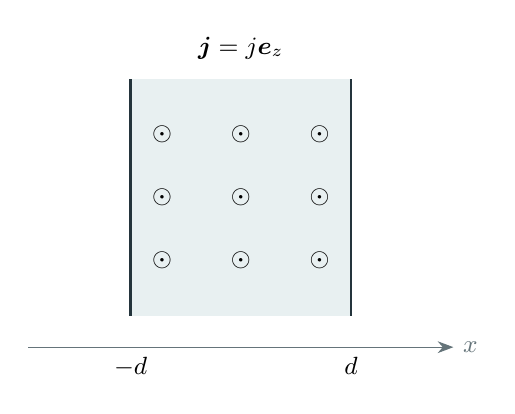
\begin{tikzpicture}[x=1cm,y=1cm]
\fill[accent!10] (-1.4,-1.5) rectangle(1.4,1.5);\draw[object] (-1.4,-1.5)--(-1.4,1.5);\draw[object] (1.4,-1.5)--(1.4,1.5);\foreach \x in {-1,0,1}\foreach \y in {-.8,0,.8}\node at (\x,\y) {$\odot$};\draw[axis] (-2.7,-1.9)--(2.7,-1.9) node[right] {$x$};\node[below] at (-1.4,-1.9) {$-d$};\node[below] at (1.4,-1.9) {$d$};\node at (0,1.9) {$\vect j=j\vect e_z$};
\end{tikzpicture}\figcaption{图电2.6　截面中圆点表示向外的电流；层沿y和z无限延伸。}\end{minipage}\end{center}

\workarea

\clearpage

\pdfbookmark[2]{第 7 题 载流圆柱内的电子收缩与净电荷}{q7}

\section*{第 7 题\quad 载流圆柱内的电子收缩与净电荷}\label{q:7}

无限长圆柱导体未通电时，电子体电荷密度为$\rho_0<0$，固定正离子体电荷密度为$-\rho_0$。通电后电子以均匀轴向漂移速率$u<c$运动，磁力使电子趋向中轴，产生径向电场。假定电子在所占据的轴对称体区域内已达到电力与磁力平衡。求该区域的电子密度和净体电荷密度；说明有限截面导线中电荷守恒对边缘分布的限制。

\begin{center}\begin{minipage}{.97\linewidth}\centering
\begin{tikzpicture}[x=1cm,y=1cm,font=\small]
\fill[warm!8] (0,0) circle(1.7);
\fill[accent!10] (0,0) circle(1.36);
\draw[object] (0,0) circle(1.7);
\draw[guide] (0,0) circle(1.36);
\draw[axis] (0,0)--(2.6,0) node[right] {$r$};
\draw[<->] (0,0)--(135:1.36) node[pos=.75,below left] {$r_e$};
\draw[<->] (0,-2.05)--(1.7,-2.05) node[midway,below] {$R$};
\node at (.2,.6) {电子体区};
\node at (.15,-.55) {$\rho<0$};
\node at (0,2.2) {$\odot\,j_z>0,\qquad\otimes\,\boldsymbol u$};
\end{tikzpicture}
\figcaption{图电2.7　电子平均速度指向纸内（$-z$），常规电流指向纸外（$+z$）。外圆半径为$R$，虚圆示意待求的电子体区边界$r_e$。}
\end{minipage}\end{center}


\workarea

\clearpage

\pdfbookmark[2]{第 8 题 磁场中转杆与滑动带电环}{q8}

\section*{第 8 题\quad 磁场中转杆与滑动带电环}\label{q:8}

光滑刚性细杆在水平面内绕固定竖直轴无摩擦旋转，杆对该轴的转动惯量为$J$。质量$m$、电荷$q>0$的小环套在杆上，与杆间无电荷转移。匀强磁场$B$垂直水平面向里，正转向取逆时针。
\begin{enumerate}
\item 小环在非零半径处相对杆静止时，求杆可能的非零角速度。
\item 杆初角速度$\omega_0>qB/m$，小环起初位于轴处，受微小扰动后沿杆外移。环能否在某个非零半径处径向停下，并从此相对杆保持静止？
\item 把初角速度变成$\alpha\omega_0$（$\alpha>0$），若要保持小环的空间轨道相同，磁场大小应怎样改变？
\end{enumerate}

\begin{center}\begin{minipage}{.98\linewidth}\centering
\begin{tikzpicture}[x=1cm,y=1cm]
\draw[object] (-.8,0)--(4,0);\fill (0,0) circle(2.5pt) node[below] {转轴};\draw[fill=white,thick] (2.2,0) circle(.13);\node[above] at (2.2,.18) {$m,q$};\draw[<->] (0,-.5)--(2.2,-.5) node[midway,below] {$r$};\draw[motion] (.8,.4) arc(25:115:.9) node[above] {$\omega$};\node at (3.6,1.1) {$\otimes B$};\node at (-.6,1.3) {$J$};
\end{tikzpicture}\figcaption{图电2.8　俯视转杆，角速度正向为逆时针。}\end{minipage}\end{center}

\workarea

\clearpage

\pdfbookmark[2]{第 9 题 地磁场中带电圆环的滑动与纯滚动}{q9}

\section*{第 9 题\quad 地磁场中带电圆环的滑动与纯滚动}\label{q:9}

半径$R$、质量$m$的均匀细圆环带有相对环固定的均匀正电荷$Q$，竖立在水平地面上。初态仅有向东的平动速度$v_0>0$，没有转动。地面动摩擦因数为$\mu>0$，均匀磁场$B$沿水平方向向北。忽略电磁辐射和形变。
\begin{enumerate}
\item 求圆环始终不离开地面的$v_0$范围。
\item 在达到纯滚动之前，求平动速度$v(t)$。
\item 当$v_0=mg/(2QB)$时，求达到纯滚动的时刻。
\end{enumerate}

\begin{center}\begin{minipage}{.98\linewidth}\centering
\begin{tikzpicture}[x=1cm,y=1cm]
\draw[object] (0,1.4) circle(1.4);\draw[object] (-2,0)--(3.6,0);\fill[pattern=north east lines] (-2,-.18) rectangle(3.6,0);\draw[motion] (1.7,1.4)--(3,1.4) node[right] {$v_0$};\node at (0,1.4) {$m,Q$};\node at (-1.8,2.7) {$\otimes B$};\node at (3,-.45) {$\mu$};\node at (-.8,-.45) {西};\node at (2.2,-.45) {东};
\end{tikzpicture}\figcaption{图电2.9　环竖直放置，初始向东平动，无初始自转。}\end{minipage}\end{center}

\workarea

\clearpage

\pdfbookmark[2]{第 10 题 电子枪击靶的圆轨道与螺旋轨道}{q10}

\section*{第 10 题\quad 电子枪击靶的圆轨道与螺旋轨道}\label{q:10}

电子经$U=1000\,\mathrm V$的电压从静止加速后，从枪口$T$沿直线$a$方向射出。靶$M$到$T$的距离$d=5.0\,\mathrm{cm}$，$TM$与初速度方向夹角$\phi=60^\circ$。求下列两种磁场下能击中$M$所需的磁感应强度：
\begin{enumerate}\item 磁场垂直于$a$和$TM$所在平面；选取使电子向靶偏转的方向。
\item 磁场平行$TM$，方向由$T$指向$M$。\end{enumerate}
电子质量$m_e=9.11\times10^{-31}\,\mathrm{kg}$，电荷绝对值$e=1.60\times10^{-19}\,\mathrm C$，采用非相对论近似。

\begin{center}\begin{minipage}{.98\linewidth}\centering
\begin{tikzpicture}[x=1cm,y=1cm]
\coordinate (T) at (0,1);\coordinate (M) at (1.5,-1.598);\draw[object] (-1.2,.85)--(0,.85)--(0,1.15)--(-1.2,1.15);\draw[motion] (T)--(2,1) node[right] {$v$};\draw[guide] (T)--(M) node[midway,below left] {$d$};\fill (M) circle(2pt) node[right] {$M$};\node[above] at (T) {$T$};\draw (.6,1) arc(0:-60:.6);\node at (.9,.72) {$\phi$};\node[right] at (3,1) {$a$};
\end{tikzpicture}\figcaption{图电2.10　目标方向与枪口初速度夹角为$\phi$。}\end{minipage}\end{center}

\workarea

\clearpage

\pdfbookmark[2]{第 11 题 平移细管内出射粒子追碰目标}{q11}

\section*{第 11 题\quad 平移细管内出射粒子追碰目标}\label{q:11}

纸面内有长$h$的光滑绝缘细管$MN$，$M$在下、$N$在上。管内小球$P_1$质量$m$、电荷$q>0$，初始相对管静止在$M$；不带电小球$P_2$初始在$N$口外（与初始$N$坐标重合），沿水平向左作匀速运动，速率$u_2$。从$t=0$起细管以水平向右恒速$u_1>0$平移，管不转动，管质量足够大，忽略$P_1$对管运动的影响。匀强磁场$B$垂直纸面向里。求$P_1$从$N$射出后最终与$P_2$相碰所允许的$u_2$。忽略重力；出管后不再受管的约束。

\begin{center}\begin{minipage}{.98\linewidth}\centering
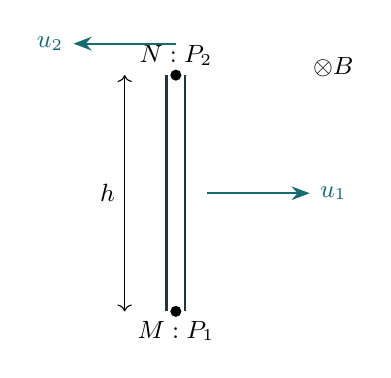
\begin{tikzpicture}[x=1cm,y=1cm]
\draw[object] (-.12,-1.5)--(-.12,1.5);\draw[object] (.12,-1.5)--(.12,1.5);\fill (0,-1.5) circle(2pt) node[below] {$M:P_1$};\fill (0,1.5) circle(2pt) node[above] {$N:P_2$};\draw[motion] (.4,0)--(1.7,0) node[right] {$u_1$};\draw[motion] (0,1.9)--(-1.3,1.9) node[left] {$u_2$};\draw[<->] (-.65,-1.5)--(-.65,1.5) node[midway,left] {$h$};\node at (2,1.6) {$\otimes B$};
\end{tikzpicture}\figcaption{图电2.11　初态两球分别位于细管两端，管向右而目标向左。}\end{minipage}\end{center}

\workarea

\clearpage

\pdfbookmark[2]{第 12 题 方波轴向磁场中的电子束聚焦}{q12}

\section*{第 12 题\quad 方波轴向磁场中的电子束聚焦}\label{q:12}

半径$R$的圆筒真空管中，两个有轴心小孔$A,A'$的隔板相距$L$。左侧电子枪连续发出电子，经$A$进入两隔板间的区域，所有电子的轴向速度分量均为$v$，横向速度各不相同。忽略电子间作用，碰壁电子被吸收。恒定轴向磁场中，使电子束在$A'$重新聚焦的最小场强为$B_0$。现令该区域磁场在$+B_0$、$-B_0$间交替，每半周期翻转一次，$t=0$起为正。
\begin{enumerate}
\item 求使非轴向电子能够在$A^{\prime}$重新聚焦的最小变化周期$T_0$。
\item 若$T=2T_0$，标出非轴向电子经$A'$射出的时间区间。
\item 求通过$A'$的电子出射方向与管轴夹角的上限。
\end{enumerate}
采用理想磁偏转模型，忽略翻转阶段的感生电场和过渡时间。

\begin{center}\begin{minipage}{.98\linewidth}\centering
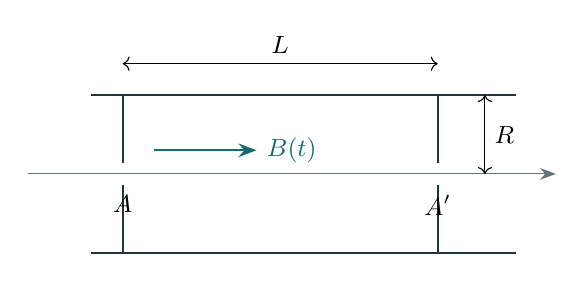
\begin{tikzpicture}[x=1cm,y=1cm]
\draw[object] (-.4,1)--(5,1);\draw[object] (-.4,-1)--(5,-1);\foreach \x/\t in {0/A,4/{A'}}{\draw[object] (\x,-1)--(\x,-.14);\draw[object] (\x,.14)--(\x,1);\node[below] at (\x,-.15) {$\t$};}\draw[axis] (-1.2,0)--(5.5,0);\draw[motion] (.4,.3)--(1.7,.3) node[right] {$B(t)$};\draw[<->] (0,1.4)--(4,1.4) node[midway,above] {$L$};\draw[<->] (4.6,0)--(4.6,1) node[midway,right] {$R$};
\end{tikzpicture}\figcaption{图电2.12　两隔板间为方波轴向磁场；两小孔均在轴线上。}\end{minipage}\end{center}

\workarea

\clearpage

\pdfbookmark[2]{第 13 题 同轴磁控管的临界磁场}{q13}

\section*{第 13 题\quad 同轴磁控管的临界磁场}\label{q:13}

无限长同轴导体间为真空，内圆柱半径$a$，外圆柱内半径$b>a$，外极相对内极电势为$V\ge0$。匀强磁场$\vect B=B\vect e_z$沿轴线向外。电子质量$m$、电荷$-e$，忽略空间电荷和感应电荷。
\begin{enumerate}
\item $B=0$，电子从内极无初速逸出，求到外极的速率，分别给出非相对论与相对论结果。
\item $V=0$，电子从内极以径向初速$v_0$逸出，求恰能触及外极的临界场，并画略强于临界时的轨道。
\item 求机械角动量$L_z$的变化率，证明$L_z-keBr^2$守恒并确定$k$。
\item 无初速电子若不能到达外极，求在最大半径$r_{\max}$处速率与$r_{\max}$的关系。
\item $V>0$时，求阻止无初速电子到达外极的临界磁场。
\item 电子从内极逸出时，沿轴、径向向外、逆时针切向初速分别为$v_z,v_r,v_\phi$，求正向磁场的临界值。
\end{enumerate}
除第(1)问相对论结果外，其余均采用非相对论近似。

\begin{center}\begin{minipage}{.98\linewidth}\centering
\begin{tikzpicture}[x=1cm,y=1cm]
\draw[object] (0,0) circle(2);\fill[accent!15] (0,0) circle(.7);\draw[object] (0,0) circle(.7);\draw[axis] (0,0)--(2.7,0) node[right] {$r$};\node[above] at (.7,0) {$a$};\node[above] at (2,0) {$b$};\node at (-.9,2.2) {$\odot B$};\node at (0,-.35) {内极};\node at (0,-2.4) {外极：$+V$};\draw[motion] (.7,0)--(1.25,0) node[above] {$v_r$};
\end{tikzpicture}\figcaption{图电2.13　电势从内极向外极升高，电子带负电。}\end{minipage}\end{center}

\workarea

\clearpage

\pdfbookmark[2]{第 14 题 点源到点像的磁场边界}{q14}

\section*{第 14 题\quad 点源到点像的磁场边界}\label{q:14}

质量$m$、正电荷$q$的离子从$P=(-a,0)$以相同速率$v$向$xy$上半平面的各方向射出。设计一块垂直纸面的匀强磁场$B$，使可接收的离子聚焦到$R=(a,0)$；轨道关于$y$轴对称。求磁场边界，并讨论回转半径$r=mv/(qB)$小于、等于、大于$a$时的接收角范围。出射角$\phi$从正$x$方向量起。

\begin{center}\begin{minipage}{.98\linewidth}\centering
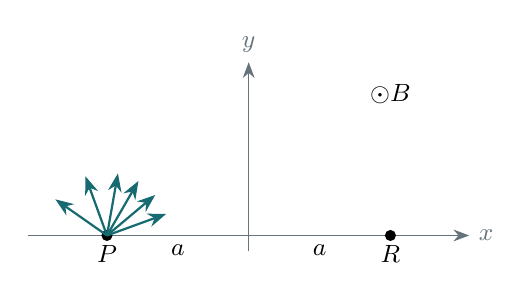
\begin{tikzpicture}[x=1cm,y=1cm]
\draw[axis] (-2.8,0)--(2.8,0) node[right] {$x$};\draw[axis] (0,-.2)--(0,2.2) node[above] {$y$};\fill (-1.8,0) circle(2pt) node[below] {$P$};\fill (1.8,0) circle(2pt) node[below] {$R$};\foreach \ang in {20,40,60,80,110,145}\draw[motion] (-1.8,0)--++(\ang:.8);\node[below] at (-.9,0) {$a$};\node[below] at (.9,0) {$a$};\node at (1.8,1.8) {$\odot B$};
\end{tikzpicture}\figcaption{图电2.14　从P发射的上半平面点源，设计左右对称场区。}\end{minipage}\end{center}

\workarea

\clearpage

\pdfbookmark[2]{第 15 题 电子束先会聚再扩束的四区磁场}{q15}

\section*{第 15 题\quad 电子束先会聚再扩束的四区磁场}\label{q:15}

一束稀疏电子从$x$负半轴远处、$-H<y<H$的条带中，以同一速率$v$沿正$x$方向平行入射。设计有限的分区匀强磁场，使所有电子先通过原点$O$，再在远处恢复为沿正$x$方向、同一速率$v$的平行束，出射条带为$-2H<y<2H$。忽略电子间相互作用，给出一种场区边界及各区磁场。

\begin{center}\begin{minipage}{.98\linewidth}\centering
\begin{tikzpicture}[x=1cm,y=1cm]
\draw[axis] (-3.2,0)--(4.3,0) node[right] {$x$};\draw[axis] (0,-2.4)--(0,2.4) node[above] {$y$};\foreach \y in {-.8,-.4,.4,.8}\draw[motion] (-3,\y)--(-1.9,\y);\foreach \y in {-1.6,-.8,.8,1.6}\draw[motion] (2.1,\y)--(3.2,\y);\draw[<->] (-2.9,-1)--(-2.9,1) node[pos=.70,left] {$2H$};\draw[<->] (3.1,-2)--(3.1,2) node[pos=.60,right] {$4H$};\node[below left] at (0,0) {$O$};
\end{tikzpicture}\figcaption{图电2.15　入射束半宽H，要求过O后成为半宽2H的平行束。}\end{minipage}\end{center}

\workarea

\clearpage

\pdfbookmark[2]{第 16 题 环形磁场中的电子束聚焦与漂移}{q16}

\section*{第 16 题\quad 环形磁场中的电子束聚焦与漂移}\label{q:16}

平均半径$R$的螺绕环中，从场线上的点源$P$沿磁力线方向射入小孔径角$2\alpha_0$的电子束，$\alpha_0\ll1$。电子均经电压$U_0$加速，忽略相互作用。磁场大小按理想模型取常量$B$。
\begin{enumerate}
\item 求使电子沿半径$R$的圆形轴线运动所需的垂直环平面匀强偏转场$B_1$。
\item 忽略$B_1$和场线弯曲，要求电子束每绕环$\pi/2$圆周角聚焦一次，求$B$。
\item 不加$B_1$，电子沿环切线发射。证明其径向偏离有界，并确定垂直环面的漂移方向；保留径向转向方程及其精确求根形式。
\end{enumerate}
给定$e/m=1.76\times10^{11}\,\mathrm{C/kg}$、$U_0=3\,\mathrm{kV}$、$R=50\,\mathrm{mm}$。取环面为$xy$面、环形场沿$+\phi$方向。

\begin{center}\begin{minipage}{.98\linewidth}\centering
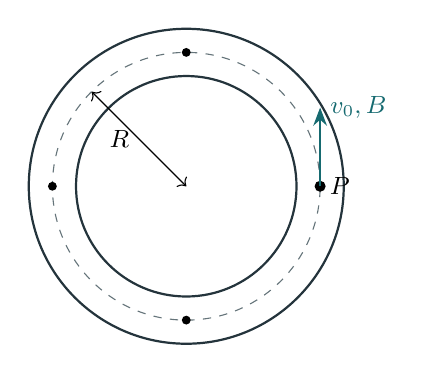
\begin{tikzpicture}[x=1cm,y=1cm]
\draw[object] (0,0) circle(2);\draw[object] (0,0) circle(1.4);\draw[guide] (0,0) circle(1.7);\fill (1.7,0) circle(2pt) node[right] {$P$};\draw[motion] (1.7,0)--(1.7,1) node[right] {$v_0,B$};\draw[<->] (0,0)--(-1.2,1.2) node[midway,left] {$R$};\foreach \ang in {90,180,270}\fill (\ang:1.7) circle(1.6pt);
\end{tikzpicture}\figcaption{图电2.16　沿环形轴线每四分之一周设置一个近轴焦点。}\end{minipage}\end{center}

\workarea

\clearpage

\pdfbookmark[2]{第 17 题 磁铁边缘场的单平面聚焦}{q17}

\section*{第 17 题\quad 磁铁边缘场的单平面聚焦}\label{q:17}

两平面磁极沿$z$方向长$L$，极间距远小于$L$，内部近似匀强场$B_0\vect e_x$，出口边缘磁力线弯曲。$yz$面为两极中分面。正电荷$q$的粒子从$x=x_0$处沿$+z$方向入射，初动量$p_0\gg qB_0L$，且$|x_0|$远小于极间距。
\begin{enumerate}\item 求穿过磁铁后$yz$平面的小偏转角$\theta_y$。
\item 证明出口边缘使$xz$平面转角近似$\theta_x=-x_0\theta_y^2/L$。
\item 证明不同$x_0$的平行束在$xz$投影中聚焦，求出口后的焦距，并说明三维轨道是否落在$z$轴上。\end{enumerate}

\begin{center}\begin{minipage}{.98\linewidth}\centering
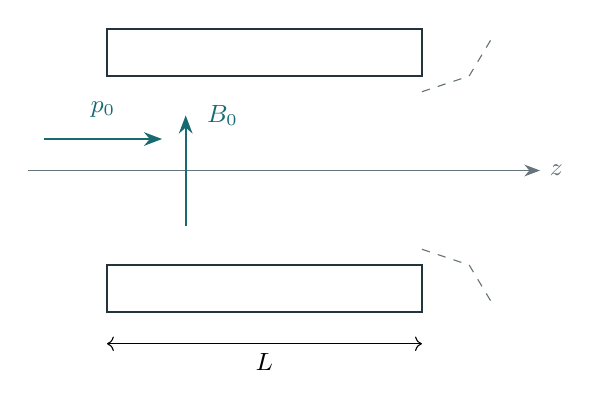
\begin{tikzpicture}[x=1cm,y=1cm]
\draw[object] (0,1.2)--(4,1.2)--(4,1.8)--(0,1.8)--cycle;\draw[object] (0,-1.2)--(4,-1.2)--(4,-1.8)--(0,-1.8)--cycle;\draw[axis] (-1,0)--(5.5,0) node[right] {$z$};\draw[motion] (1,-.7)--(1,.7) node[right=4pt] {$B_0$};\draw[motion] (-.8,.4)--(.7,.4) node[midway,above=4pt] {$p_0$};\draw[guide] (4,1)--(4.6,1.2)--(4.9,1.7);\draw[guide] (4,-1)--(4.6,-1.2)--(4.9,-1.7);\draw[<->] (0,-2.2)--(4,-2.2) node[midway,below] {$L$};
\end{tikzpicture}\figcaption{图电2.17　示意xz截面内的主磁场和出口边缘场。}\end{minipage}\end{center}

\workarea

\clearpage

\pdfbookmark[2]{第 18 题 电场漂移与磁场梯度漂移}{q18}

\section*{第 18 题\quad 电场漂移与磁场梯度漂移}\label{q:18}

粒子从$O$以$v_0\vect e_y$发射，质量$m$、电荷$q\ne0$，忽略重力。
\begin{enumerate}
\item 在$B\vect e_z$的匀强磁场中叠加弱匀强电场$E\vect e_y$，分别判断$q>0$、$q<0$的漂移方向，并求漂移速率。
\item 不要求$E$弱，严格求$v_x(t),v_y(t)$，初始时刻$t=0$。
\item 撤去电场，令磁场大小沿$+y$方向有微小正梯度，定性判断两种电荷的漂移方向，并给出弱梯度近似的表达式。
\end{enumerate}

\begin{center}\begin{minipage}{.98\linewidth}\centering
\begin{tikzpicture}[x=1cm,y=1cm]
\draw[axis] (-2,0)--(3,0) node[right] {$x$};\draw[axis] (0,-1.2)--(0,2.4) node[above] {$y$};\draw[motion] (0,0)--(0,1) node[left] {$v_0$};\draw[force] (.5,.2)--(.5,1.3) node[right] {$E$};\node at (-1.4,1.5) {$\odot B$};\fill (0,0) circle(1.5pt) node[below left] {$O$};
\end{tikzpicture}\figcaption{图电2.18　电场沿正y轴，磁场沿正z轴。}\end{minipage}\end{center}

\workarea

\clearpage

\pdfbookmark[2]{第 19 题 重力与磁场中同高度的再相遇}{q19}

\section*{第 19 题\quad 重力与磁场中同高度的再相遇}\label{q:19}

足够大的匀强磁场$B$水平且垂直纸面向里。质量$m$、电荷$q>0$的粒子，从点$a$以水平向右初速度$v_0>0$射向同高度点$b$，$ab=s>0$。重力加速度为$g$。求能使粒子经过$b$的全部初速度，并说明特殊间距的意义。

\begin{center}\begin{minipage}{.98\linewidth}\centering
\begin{tikzpicture}[x=1cm,y=1cm]
\draw[guide] (-.3,0)--(5,0);\fill (0,0) circle(2pt) node[below] {$a$};\fill (4.4,0) circle(2pt) node[below] {$b$};\draw[motion] (0,0)--(1.3,0) node[above] {$v_0$};\draw[force] (0,-.3)--(0,-1.2) node[right] {$mg$};\node at (3,1.2) {$\otimes B$};\draw[<->] (0,-1.7)--(4.4,-1.7) node[midway,below] {$s$};
\end{tikzpicture}\figcaption{图电2.19　重力向下而正电荷初始磁力向上。}\end{minipage}\end{center}

\workarea

\clearpage

\pdfbookmark[2]{第 20 题 载流双杆与弹簧的小振动}{q20}

\section*{第 20 题\quad 载流双杆与弹簧的小振动}\label{q:20}

两根平行金属棒各长$L$、质量$m$，上下两端由两根相同轻金属弹簧连接成闭合回路，每根弹簧劲度系数$k$、原长$\ell_0\ll L$。两棒只能在水平面作左右对称的平移，边缘效应及自感忽略。外部维持恒定电流$I$，两棒电流方向相反。求平衡间距及围绕平衡位置作小振动的周期。

\begin{center}\begin{minipage}{.98\linewidth}\centering
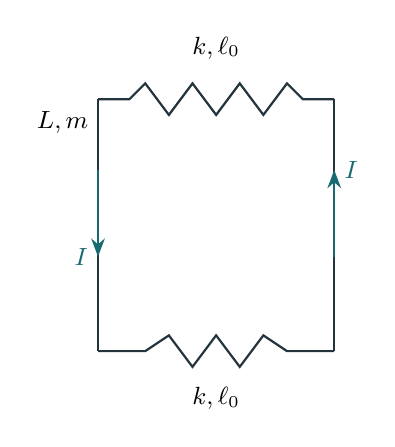
\begin{tikzpicture}[x=1cm,y=1cm]
\draw[object] (-1.5,-1.6)--(-1.5,1.6);\draw[object] (1.5,-1.6)--(1.5,1.6);\draw[object] (-1.5,1.6)--(-1.1,1.6)--(-.9,1.8)--(-.6,1.4)--(-.3,1.8)--(0,1.4)--(.3,1.8)--(.6,1.4)--(.9,1.8)--(1.1,1.6)--(1.5,1.6);\draw[object] (-1.5,-1.6)--(-.9,-1.6)--(-.6,-1.4)--(-.3,-1.8)--(0,-1.4)--(.3,-1.8)--(.6,-1.4)--(.9,-1.6)--(1.5,-1.6);\draw[motion] (-1.5,.7)--(-1.5,-.4) node[left] {$I$};\draw[motion] (1.5,-.4)--(1.5,.7) node[right] {$I$};\node at (0,2.25) {$k,\ell_0$};\node at (0,-2.2) {$k,\ell_0$};\node[left] at (-1.5,1.3) {$L,m$};
\end{tikzpicture}\figcaption{图电2.20　两杆电流反向，弹簧并联提供横向回复力。}\end{minipage}\end{center}

\workarea

\clearpage

\pdfbookmark[2]{第 21 题 旋转带电圆环的附加张力}{q21}

\section*{第 21 题\quad 旋转带电圆环的附加张力}\label{q:21}

半径$R$、质量$m$的均匀细圆环带有固定在环上的均匀正电荷$Q$，放在光滑水平面上。匀强磁场$B$垂直向上。圆环绕过圆心的竖直轴以角速度$\omega$逆时针匀速旋转，形状保持不变。求相对于同一圆环静止时，由旋转引起的附加张力；不计形变及旋转电荷的自磁场。

\begin{center}\begin{minipage}{.98\linewidth}\centering
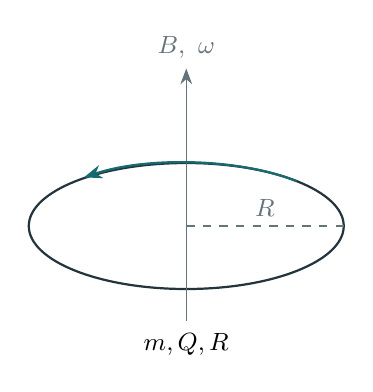
\begin{tikzpicture}[x=1cm,y=1cm]
\draw[object] (0,0) ellipse(2 and .8);\draw[axis] (0,-1.2)--(0,2) node[above] {$B,\ \omega$};\draw[motion] (1.4,.57) arc(45:130:2 and .8);\node at (0,-1.5) {$m,Q,R$};\draw[guide] (0,0)--(2,0) node[midway,above] {$R$};
\end{tikzpicture}\figcaption{图电2.21　磁场和角速度都竖直向上。}\end{minipage}\end{center}

\workarea

\clearpage

\pdfbookmark[2]{第 22 题 圆电流对共面长直导线的作用力}{q22}

\section*{第 22 题\quad 圆电流对共面长直导线的作用力}\label{q:22}

无限长直导线与半径$R$的圆线圈共面，圆心距直导线$L>R$。直导线电流$I_1$向上，圆线圈电流$I_2$顺时针，使其靠近直导线的一侧也向上。求圆线圈对整根长直导线的作用力。

\begin{center}\begin{minipage}{.98\linewidth}\centering
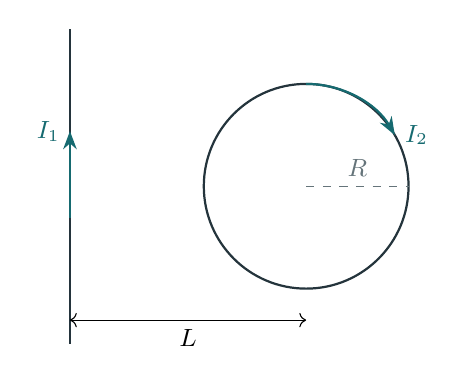
\begin{tikzpicture}[x=1cm,y=1cm]
\draw[object] (-2,-2)--(-2,2);\draw[motion] (-2,-.4)--(-2,.7) node[left] {$I_1$};\draw[object] (1,0) circle(1.3);\draw[motion] (1,1.3) arc(90:30:1.3) node[right] {$I_2$};\draw[<->] (-2,-1.7)--(1,-1.7) node[midway,below] {$L$};\draw[guide] (1,0)--(2.3,0) node[midway,above] {$R$};
\end{tikzpicture}\figcaption{图电2.22　顺时针圆电流的近侧电流与直导线同向。}\end{minipage}\end{center}

\workarea

\clearpage

\pdfbookmark[2]{第 23 题 闭合稳恒电流回路间的作用与反作用}{q23}

\section*{第 23 题\quad 闭合稳恒电流回路间的作用与反作用}\label{q:23}

真空中有两个互不相交的任意闭合细线回路$C_1,C_2$，分别通恒定电流$I_1,I_2$。证明两回路间总磁力满足牛顿第三定律。须区分电流元之间的力与整条闭合回路的合力。

\begin{center}\begin{minipage}{.97\linewidth}\centering
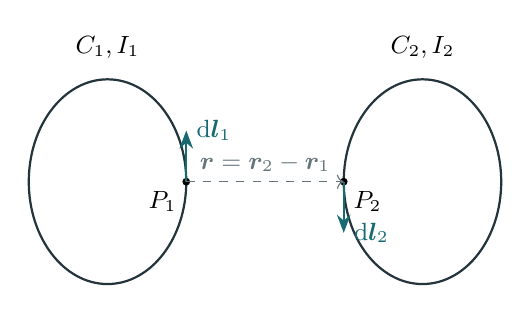
\begin{tikzpicture}[x=1cm,y=1cm,font=\small]
\draw[object] (-2,0) ellipse(1 and 1.3);\draw[object] (2,0) ellipse(1 and 1.3);
\fill (-1,0) circle(1.4pt) node[below left] {$P_1$};\fill (1,0) circle(1.4pt) node[below right] {$P_2$};
\draw[motion] (-1,0)--(-1,.65) node[right] {$\dd\boldsymbol l_1$};
\draw[motion] (1,0)--(1,-.65) node[right] {$\dd\boldsymbol l_2$};
\draw[guide,->] (-1,0)--(1,0) node[midway,above] {$\boldsymbol r=\boldsymbol r_2-\boldsymbol r_1$};
\node at (-2,1.7) {$C_1,I_1$};\node at (2,1.7) {$C_2,I_2$};
\end{tikzpicture}
\figcaption{图电2.23　两个互不相交的闭合回路；电流元在当地切线上，r从回路1的源点指向回路2的场点。}
\end{minipage}\end{center}

\workarea

\clearpage

\pdfbookmark[2]{第 24 题 超导平板上方电流环的悬浮与振动}{q24}

\section*{第 24 题\quad 超导平板上方电流环的悬浮与振动}\label{q:24}

水平无限超导平板位于$z=0$，平衡后内部磁感应强度为零。质量$m$、半径$r$的均匀细电流环水平悬浮在$z=h$，其中$r\gg h$；环中稳恒电流为$I$。采用局部平行直线电流近似，并在微振动中将$I$视为恒定。
\begin{enumerate}\item 求维持悬浮的电流。
\item 环保持水平作微小上下振动，求周期$T_1$。
\item 固定一条水平直径$P_1P_2$，让环绕此直径小角摆动，求周期$T_2$。\end{enumerate}

\begin{center}\begin{minipage}{.98\linewidth}\centering
\begin{tikzpicture}[x=1cm,y=1cm]
\draw[fill=accent!8] (-2.7,-.2)--(1.8,-.2)--(2.7,.4)--(-1.8,.4)--cycle;\draw[object] (0,1.6) ellipse(1.8 and .6);\draw[guide] (0,0)--(0,1.6);\draw[<->] (2.2,.2)--(2.2,1.6) node[midway,right] {$h$};\node at (0,2.7) {$m,r,I$};\node at (0,-.6) {超导平板};
\end{tikzpicture}\figcaption{图电2.24　水平环高h，r远大于h。}\end{minipage}\end{center}

\workarea

\clearpage

\pdfbookmark[2]{第 25 题 均匀磁化长棒侧面的场边界}{q25}

\section*{第 25 题\quad 均匀磁化长棒侧面的场边界}\label{q:25}

柱形长磁棒的横截面可以是任意形状，沿长度方向均匀磁化，磁化强度为$\vect M$且平行柱轴。取长度中部的横截面，在侧面同一个光滑点的内、外无限邻近处分别取1、2，无自由面电流。证明$\vect H_1=\vect H_2$而$\vect B_1\ne\vect B_2$。说明中截面镜像对称性和边界条件各自的作用。

\begin{center}\begin{minipage}{.98\linewidth}\centering
\begin{tikzpicture}[x=1cm,y=1cm]
\draw[fill=accent!12] (-2.5,-.8) rectangle(2.5,.8);\draw[motion] (-1.7,0)--(-.5,0) node[above] {$\vect M$};\draw[motion] (.6,0)--(1.8,0);\draw[guide] (0,-1.4)--(0,1.6) node[above] {中截面};\fill (0,.65) circle(1.5pt) node[right] {$1$};\fill (0,.95) circle(1.5pt) node[right] {$2$};
\end{tikzpicture}\figcaption{图电2.25　棒轴沿水平方向，1、2在侧面内外且位于中截面。}\end{minipage}\end{center}

\workarea

\clearpage

\pdfbookmark[2]{第 26 题 均匀磁化球壳在球心的磁场}{q26}

\section*{第 26 题\quad 均匀磁化球壳在球心的磁场}\label{q:26}

内、外半径分别为$R_1,R_2$的同心球壳磁介质，在$R_1<r<R_2$内有均匀磁化强度$\vect M$，球心空腔和外部为真空，无外加场。分别用等效磁荷法和均匀磁化实心球叠加法求球心磁感应强度。

\begin{center}\begin{minipage}{.98\linewidth}\centering
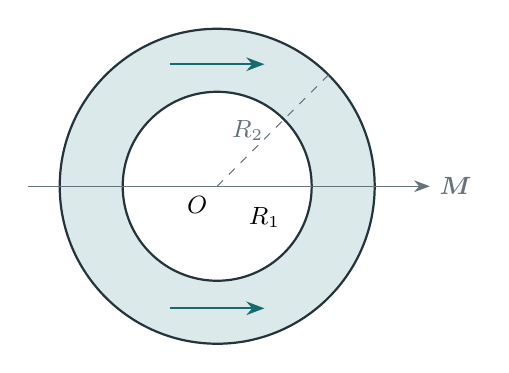
\begin{tikzpicture}[x=1cm,y=1cm]
\fill[accent!15] (0,0) circle(2);\fill[white] (0,0) circle(1.2);\draw[object] (0,0) circle(2);\draw[object] (0,0) circle(1.2);\draw[axis] (-2.4,0)--(2.7,0) node[right] {$\vect M$};\draw[guide] (0,0)--(1.414,1.414) node[midway,left] {$R_2$};\node at (.6,-.4) {$R_1$};\node[below left] at (0,0) {$O$};\foreach \y in {1.55,-1.55}\draw[motion] (-.6,\y)--(.6,\y);
\end{tikzpicture}\figcaption{图电2.26　磁化强度在球壳中均匀，球心空腔没有磁化材料。}\end{minipage}\end{center}

\workarea

\clearpage

\pdfbookmark[2]{第 27 题 旋转径向极化圆柱的场能量}{q27}

\section*{第 27 题\quad 旋转径向极化圆柱的场能量}\label{q:27}

永久极化的非磁性电介质制成半径$R$的无限长圆柱，柱内极化强度为$\vect P=\alpha r\vect e_r$，其中$\alpha>0$，柱外真空，无自由电荷，无外加电场和磁场。忽略转动引起的相对论修正和材料极化改变。
\begin{enumerate}\item 静止时，求柱内外的电场与电场能量密度。
\item 圆柱以角速度$\omega\vect e_z$绕轴匀速转动时，求柱内外的磁场与磁场能量密度。
\end{enumerate}
本题场能量指电磁场本身的$\varepsilon_0E^2/2$与$B^2/(2\mu_0)$，不包含维持永久极化和转动所需的材料机械能。

\begin{center}\begin{minipage}{.98\linewidth}\centering
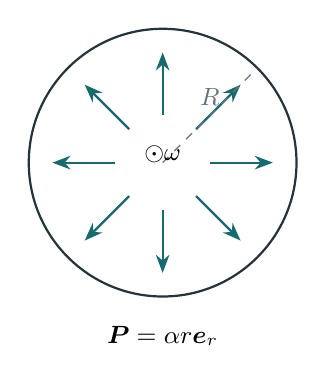
\begin{tikzpicture}[x=1cm,y=1cm]
\draw[object] (0,0) circle(1.7);\foreach \ang in {0,45,...,315}\draw[motion] (\ang:.6)--(\ang:1.4);\draw[guide] (0,0)--(1.2,1.2) node[midway,above] {$R$};\node at (0,-2.2) {$\vect P=\alpha r\vect e_r$};\node at (0,.1) {$\odot\omega$};
\end{tikzpicture}\figcaption{图电2.27　径向永久极化随半径增加，转轴垂直截面。}\end{minipage}\end{center}

\workarea

\end{document}
